\documentclass[12pt]{article}

% Language setting
% Replace `english' with e.g. `spanish' to change the document language
\usepackage[english]{babel}

% Set page size and margins
% Replace `letterpaper' with `a4paper' for UK/EU standard size

\usepackage[top=3cm,bottom=3cm,left=3cm,right=3cm,marginparwidth=1.75cm]{geometry}
	
% Load the setspace package
\usepackage{setspace}

% Useful packages
\usepackage{amsmath}
\usepackage{graphicx}
\usepackage[colorlinks=true, allcolors=blue]{hyperref}
\usepackage{tikz}
\usepackage{natbib}
\doublespacing
\bibliographystyle{unsrtnat}

\usetikzlibrary{shapes.arrows, positioning, arrows.meta}


\title{Theoretical framework}
\author{Riccardo Dal Cero}

\begin{document}
\maketitle

\begin{abstract}
    The main idea is to study how and whether the asymmetry of information have an impact on the cleansing effect of
    recession, replicating the model in computer  simulation.
\end{abstract}

\section[short]{Theoretical framework}
The economy comprises risk-neutral firms with a constant discount rate represented by $0 < \beta < 1$. These firms
exhibit heterogeneity in productivity and net worth. They employ a production technology that relies solely on capital
(or production units) as input, featuring diminishing returns to scale.
\\
In each period, firms incur a fixed production cost denoted as $c$ to initiate production. After production, they decide
how to allocate profits for the next period. The remaining profits are invested in a risk-free asset. Firms face a
choice: they can either continue operating and reinvest their profits or exit the market, investing their entire net
worth, denoted as $e$, in the risk-free asset.
\\
Firms opt to exit the market when expected profits no longer outweigh the fixed cost $c$, or when the value of
production becomes inferior to the value they could gain by investing in the risk-free asset.
\\
The value obtained from investing in the risk-free asset is given by:
\[
q_t + \sum_{s=0}^{+\infty}\beta^s[\beta(1+r)-1]e_{t+s+1}.
\]

Notably, when the condition $\beta(1+r) \leq 1$ holds, this value simplifies to $q$. In such cases, firms are either
indifferent regarding the timing of dividend distributions or have a preference for distributing their end-of-period net
worth to shareholders or investors.
\\
In this economic model, the agents are the firms themselves, aiming to maximize their value over time by selecting an
optimal level of capital denoted as $k$. The production function, accounting for the fixed cost $c$, is expressed as
follows: $Y = Z(\theta + \epsilon)k^\alpha$.
\\
Key variables include:
\begin{itemize}
    \item $Z$: Stochastic aggregate productivity common across firms.
    \item $\theta$: Persistent firm-specific productivity shock (modeled as a Markov Chain).
    \item $\epsilon$: Firm-specific productivity shock with $\epsilon \sim \mathcal{N}(0,\delta)$.
    \item $k^\alpha$: Capital or production units, as in Caballero and Hammour (AER).
\end{itemize}

The timeline of events is as follows:

\begin{figure}[h]
    \centering
    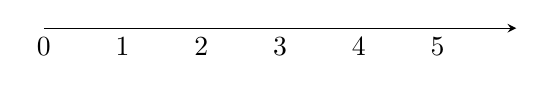
\begin{tikzpicture}
        % Draw timeline
        \draw[->,>=stealth] (0,0) -- (6,0);
        
        % Add timeline labels
        \foreach \x/\label in {0,1, 2,3, 4, 5} {
            \node[align=center, below] at (\x,0) {\label};
        }
    \end{tikzpicture}
    \caption{Timeline of Events}
\end{figure}

The sequence of events includes:
\begin{enumerate}
    \item The firm possesses knowledge of $Z,\theta,k^\alpha,e$ (where $e$ represents its endowment, different from $k$ since the firm can borrow money with $d=c+k-e$).
    \item The firm computes the optimal $k$ to maximize the expected value of the firm, with $k$ ranging from $[0,+\infty]$. If $k=0$, it indicates the firm's decision to exit.
    \item At the end of the period, the firm observes $\epsilon$ and the aggregate shock.
    \item The firm repays its debt and the fixed operating cost $(c+k-e)$, resulting in an end-of-period net worth $q$.
    \item The firm decides on the amount of dividends to distribute $(q-e')$, observes the productivity shock $\theta', Z'$, and the process restarts from step 1.
\end{enumerate}

\subsection{Frictionless economy}
In a frictionless economy, firms have the option to borrow an amount denoted as \(c+k-e\) at the risk-free interest rate
\(r=\frac{1}{\beta}-1\). Therefore, at the start of the period, the firm's value is determined by the following
expression:

\[V_{FL} = \max_{k} E \int \max[q,\max_{e'}(q - e' + \beta V_{FL}(e',\theta', Z'))]  \,d\Phi
(\epsilon) \]
where the end of period net worth is equal to:
\[q=Z(\theta+\epsilon)k^\alpha + (1-\delta )k-(1+r)(c+k-e)\]

Under the condition of survival, it can be demonstrated that:

\[\widehat{V}_{FL}(\theta,Z) = \max_{k}E\int[Z(\theta+\epsilon)k^\alpha - (1+r)c\,d\Phi (\epsilon)] +
\beta\max[0,\widehat{V}_{FL}(\theta',Z')]\]

In the absence of market frictions, firms choose to exit when their productivity reaches a certain threshold.
Specifically, they exit if \(\theta'<\underline{\theta} _{FL}(Z')\), where \(\underline{\theta}
_{FL}(Z')\) is defined as the value
for which \(\widehat{V}_{FL}(\underline{\theta}_{FL},Z')=0\).

\subsection{Economy with Credit Market Frictions}

After production, the firm privately observes the temporary shock $\epsilon$, while financial intermediaries can only
observe it at a cost of $\mu k^\alpha$. For one-period debt contracts, financial intermediaries observe $\epsilon$ only
if the firm faces financial distress, which occurs when the private shock is insufficient to repay its debt. The terms
of the financial contract depend on the firm's net worth $e$, current productivity $\theta$, and aggregate productivity
value $Z$, all observable by both the financial intermediary and the firm at no additional cost.

\textbf{HP1 (Hypothesis 1):} The risk-free interest rate is $\beta < \frac{1}{1+r}$, which implies a lower risk-free
rate in an economy with credit frictions compared to a frictionless one. It also ensures that firms do not always
reinvest their profits.

When a firm defaults, the financial intermediary incurs verification costs and seizes all of the firm's income. The
default threshold $\overline{\epsilon}$ is determined by the equation:
\[
Z(\theta+\overline{\epsilon})k^\alpha + (1-\delta)k = (1+\widetilde{r} )(c+k+e)
\]

Default results in a zero net worth but does not necessarily force the firm to exit the market, depending on its
persistent productivity component $\theta$.

The financial intermediary lends $(c + k - e)$ to the firm only if the expected income from the loan equals the
opportunity cost of the funds, as expressed by the inequality:
\[
(1+\widetilde{r} )(k+c+e)(1-\Phi(\overline{\epsilon}))+\int_{-\infty}^{\overline{\epsilon}}[Z(\theta+\overline{\epsilon})
k^\alpha+(1-\delta)k-\mu k^\alpha] \,d\Phi(\epsilon) \geq (1+r)(c+k+e)
\]

The financial contract is characterized by $(k,\overline{\epsilon})$. Given $Z,\theta,e$, the participation constraint
indicates the default threshold $\overline{\epsilon}$ required by the financial intermediary to lend a given amount. For
some firms, their net worth is too low for the participation constraint of the financial intermediary to be satisfied.
In fact, given $\theta, Z$, there is a unique threshold $e_b(\theta,Z)$ below which the financial intermediary
refuses to lend any amount:
\[
Z[\theta+G(\overline{\epsilon}_b )]k^\alpha+(1-\delta)k-uk_b^\alpha\Phi (\overline{\epsilon}_b)=(1+r)(k_b+c-\underline{e_b})
\]
where $\overline{\epsilon}_b$ maximizes the expected income of the financial intermediary. When the firm has a net worth
below $\underline{e_b}$, the firm defaults.

After production, the firm's end-of-period net worth is equal to:
\[
q = \begin{cases}
  Z(\theta+\overline{\epsilon})k^\alpha +(1-\delta)k-(1+\widetilde{r})(k+c-e) & \text{if } \epsilon\geq \overline{\epsilon} \\
  0 & \text{otherwise}
\end{cases}
\]
Using the default condition we can rewrite as 
\[q = \max[Zk^\alpha(\epsilon-\overline{\epsilon});0]\]

\subsection{The firm's problem}
Define $V$ as the firm's value at the start of the period, which hinges on investment outcomes and exit decisions. If
the end-of-period net worth falls below a threshold ($q < e_b(\theta', Z')$), the firm exits. Otherwise, it compares its
continuing value to the end-of-period net worth ($q \geq e_b(\theta', Z')$) and exits if the continuing value is lower.

The firm's value function is given by:
\[
V(e,\theta,Z) = \max_{(k,\overline{\epsilon})}E\left\{\int I(q)q + (1-I(q))\max[q,\max_{e'}q-e'+\beta V(e',\theta',
\zeta')]\,d\Phi(\epsilon)\right\}
\]

Where:
\[
I(q)=
\begin{cases}
    0 & \text{if } q\geq e_b(\theta', Z')\\
    1 & \text{if } q< e_b(\theta', Z')
\end{cases}
\]

Subject to the following constraints:
\begin{enumerate}
    \item \label{con1}\[
    Z[\theta+G(\overline{\epsilon}_b )]k^\alpha+(1-\delta)k-uk_b^\alpha\Phi (\overline{\epsilon}_b)\geq(1+r)(k_b+c-
    \underline{e_b})
    \]
    \item \label{con2} \[
    q = \max[Zk^\alpha(\epsilon-\overline{\epsilon});0]
    \]
    \item \label{con3}\[
    \overline{e_b}(\theta',Z)\leq e'\leq q
    \]
\end{enumerate}

The firm aims to maximize expected dividends while complying with the financial intermediary's participation constraint
(constraint 1). Equation (constraint 2) characterizes the firm's end-of-period net worth, and
Equation (constraint 3) ensures that the
net worth
is sufficiently high to satisfy the participation constraint.
\par
Furthermore, the firm is prohibited from issuing new shares and can only augment its net worth by reinvesting profits.
This limitation presents a trade-off: increasing capital boosts production capacity but also raises the risk of default,
as the default threshold set by the financial intermediary increases with borrowed amounts.
\section{The cleansing effect by Caballero}
\subsection{Introduction}
In the first paper that rationalize the cleansing effect of recessions, authored by Ricardo J. Caballero and Mohamad L.
Hammour  \cite{CabHarm94} and published in the American Economic Review in 1998, the primary aim was to investigate how
industries respond to cyclical variations in demand. They did this by employing a vintage model of creative destruction.
The underlying concept postulates that the processes of creation and destruction within an industry partially explain
business cycles. Industries continuously experiencing creative destruction can adapt to demand fluctuations in two
ways: by adjusting the rate at which they produce new units embodying advanced techniques or by altering the
rate at which outdated units are retired. The model they used incorporated heterogeneous firms, where production units
embodied the most advanced technology at the time of their creation. The costs associated with creating new units
slowed down technology adoption, resulting in the coexistence of production units with varying vintages.
\par
Key to understanding how firms adapt to business cycles are the concepts of the creative margin and the destruction
margin. For example, a reduction in demand can be accommodated either by reducing the rate of technology adoption or by
retiring older production units. One of the primary factors determining which margin is more responsive to business
cycles is the adjustment cost. When this cost follows a linear pattern, the study shows that insulation is complete, and
the industry's response relies exclusively on its creation margin. Consequently, the creation margin becomes smoother
over time in comparison to the destruction margin, which exhibits greater responsiveness to the business cycle.
\par
Crucially, Caballero and Hammour's research \cite{BlaDia90} offers theoretical insights supported by empirical
evidence. Their findings on the cyclical nature of the destruction margin align with the studies conducted by Blanchard
and Diamond \cite{BlaDia90}, as well as Steven Davis and John Haltiwanger \cite{DavHalt92}, in their respective works
from 1990. This
convergence between theoretical framework and empirical substantiation underscores the importance of comprehending the
dynamic interplay between creative destruction and business cycles, which significantly influences how industries
respond to economic fluctuations.
\par
In their study \cite{DavHalt92}, where they assess the heterogeneity of employment changes at the establishment level in
the U.S. manufacturing sector from 1972 to 1986, it is revealed that job destruction exhibits procyclical tendencies,
responding more robustly to downturns in the economic cycle compared to the creation rate, in line with the theoretical
model proposed by Caballero and Hammour \cite{CabHarm94}. The authors leverage a natural experiment inherent in the data
to examine whether the structure of adjustment costs can account for the behavior of these two margins. This natural
experiment arises from the asymmetric nature of business cycles, with recessions being shorter but more severe than
expansions. The theoretical model predicts that these differences should be attenuated in the creation process, a
prediction that is substantiated by the data since creation exhibits relative symmetry around its mean, while
destruction displays a high degree of asymmetry.
The underlying concept driving the behavior of the destruction margin can be traced back to the theories of Schumpeter
and Hayek.  They suggest that recessions represent periods during which unprofitable or outdated techniques are pruned
from the economy, leaving behind the most efficient firms \citet{HaCa07}.
\subsection{Theoretical model}
The model in question is a vintage model that simulates an industry experiencing exogenous technological progress.
Within this model, production units are constructed using a fixed proportion of labor and capital, and they are
continually being created and phased out. Notice that only the creation of new production units
incurs a cost. This simplification is plausible, particularly in the context of the United States, where the expense
associated with hiring is typically higher than the cost of termination, as demonstrated by Abdulkadiroğlu and Kranton
(2003) \cite{AbdKra03}. 
\par
In this model, when a production unit is created at a specific time \(t_0\), it embodies the most advanced technology
available at that moment and consistently generates a uniform output represented by \(A(t_0)\) throughout its
operational lifetime. The productivity of this technology, denoted as \(A(t)\), experiences continuous growth at an
exogenously determined constant rate \(\delta \ge 0 \). This growth in technology can be interpreted in two ways: either
as the adoption of new technology or as a product innovation. In the latter scenario, a continuum of perfectly
substitutable products can yield varying levels of output.

\[\left[ f(a,t) \qquad 0\leq a \leq \overline{a}(t) \right]\]

The above function represents the cross-sectional density of the production units aged \(a\) at time \(t\), where
\(\overline{a}(t)\) is the age of the oldest production unit at time \(t\). The first assumption is that \(f(a,t)\) and
\(\overline{a}(t)\) are continuous functions. The mass of production units at time \(t\) is given by:

\[N(t) = \int_{\overline{a}(t)}^{0}f(a,t)da\]

\(N(t)\) is a measure of either the industry's capital stock and its employment, due to a fixed share of capital and
labor. Thus, the industry's output is given by:

\[Q(t) = \int_{\overline{a}(t)}^{0}A(t-a)f(a,t)da\]

The deterioration of production units involves both an exogenous depreciation rate \(\delta\) and an endogenous destruction process, which impacts \(f(a,t)\) at its limits. The count of production units surviving for \(a\) years is expressed as:

\[f(a,t)= f(0,t-a)e^{-\delta a} \quad \text{where } 0 < a \leq \overline{a}(t)\]

The production flow is determined by:

\[\dot{N}(t) = f(0,t) [1-\overline{\dot{a}}(t)] + \delta N(t)\]

Here, the first term represents the production rate, while the second term encapsulates the destruction rate, encompassing the obsolescence rate \(f(\overline{a})(t)\), the technological obsolescence change over time \(-f(\overline{a})(t)\overline{\dot{a}}(t)\), and the depreciation rate \(\delta N(t)\).

The assumptions made by the authors are denoted as \(\forall t \mid f(0,t)>0 \cup  \overline{\dot{a}}(t)<\).

The alteration in output concerning these flows is articulated as:

\[\dot{Q}(t) = A(t)f(0,t) - A(t-\overline{a}(t))f(\overline{a}(t),t) \cdot [1-\overline{\dot{a}}(t)] + \delta Q(t)\]

The authors define a perfectly competitive industry in partial equilibrium, where supply is dictated by free entry and perfect equilibrium. Additionally, they introduce a cost function related to creating new production units:

\[c = c\left(f\left(f(0,t)\right)\right) \quad \text{where } c(\cdot)>0, \, c'(\cdot)\leq 0\]

This cost function is contingent on the creation rate, implying that higher creation rates correspond to increased
costs. The equilibrium condition is established by equating the cost of unit creation to the present discounted value of
profits throughout its lifespan. The authors set the cost of a production unit to 1, and \(P(t)\) is the price of a unit
of output. Thus, the profits generated at time \(t\) by a production unit aged \(a\) are defined as: 

\[\pi(a,t)= P(t)A(t-a)-1\]
\[\overline{a}[t+T(t)] = T(t)\]

Here, \(T(t)\) signifies the maximum lfetime of a unit created at \(t\). At any given time \(t\), the free entry
condition is expressed as: 

\[ c(f(0,t)) = \int_{t+T(t)}^{t}\pi(s-t,t)e^{-(r+\delta)(s-t)\,ds} \]

In the above equation, where \(r>0\) represents the exogenously determined instantaneous interest rate, the determination of
the exit of a production unit is contingent upon continuous \(P(t)\) and the instance when the profits generated by a
unit being destroyed reach zero. This occurrence signifies the moment when the oldest unit operational at time \(t\),
denoted as \(\overline{a(t)}\), must adhere to the equation: 

\[P(t)A(t-\overline{a}(t))=1\]

The authors posit that \(P(t)\) exhibits a decreasing trend due to the model's assumption regarding endogenous
destruction, specifically \(\overline{\dot{a}(t)}<1\). To see, differentiate 
\[\dot{P}(t)=-\gamma\left[1-\overline{\dot{a}}P(t)\right]\]
Consequently, when the profits of a production unit diminish to
zero for the first time, it will be subject to destruction. 

On the demand side, the authors assume a unit-elastic demand function and consider the aggregate expenditure as
exogenous 
\(\overline{D}(t)=P(t)Q(t)\). 
The equilibrium is a path \(\left\{f(0,t),\overline{a}(t),T(t),Q(t)\right\}_{t \geq 0}\) that satisfy the following
conditions:
\begin{enumerate}
    \item \label{eq_2.1} $ \begin{aligned}[t]
        Q(t) &= \int_{\overline{a}(t)}^{0}A(t-a)f(a,t)da
    \end{aligned}$
    \item \label{eq_2.2}$ \begin{aligned}[t]
        f(a,t)&=f(0,t-a)e^{-\delta a}      
    \end{aligned}$
    \item \label{eq_2.3}$ \begin{aligned}[t]
        T(t)&=\overline{a}\left(t+T(t)\right)        
    \end{aligned}$
    \item \label{eq_2.4}$ \begin{aligned}[t]
        c(f(0,t))&=\int_{t}^{t+T(t)}\left[P(s)A(t)-1\right]e^{-(r+\delta)(s-t)}\,ds
    \end{aligned}$
    \item \label{eq_2.5}$ \begin{aligned}[t]
        P(t)A(t-\overline{a}(t)=1)
    \end{aligned}$
    \item \label{eq_2.6}$ \begin{aligned}[t]
        P(t)Q(t)=\overline{D}(t)
    \end{aligned}$
\end{enumerate}
The first three equations (\ref{eq_2.1}, \ref{eq_2.2}, \ref{eq_2.3}) and the fifth one (\ref{eq_2.5}) suffice to delineate the trajectories of \(T(t)\), \(P(t)\), and \(Q(t)\), which are determined by \(\left\{f(0,t), \overline{a}(t)\right\}\). To affirm the robustness of the conditions expressed in equations \ref{eq_2.6} and \ref{eq_2.5}, it is possible to derive these equations as first-order conditions for the maximization of a number of perfectly competitive firms holding production units.

To comprehend the functioning of endogenous destruction, let's consider a scenario with constant demand. In this case, both the destruction and creation rates change only due to supply factors. This steady state is characterized by a constant lifetime of production units \(T(t) = \overline{a}(t) = \overline{a}^*\), resulting in a time-invariant age distribution \(f(a,t) = f^*(a)\). Equation \ref{eq_2.5} implies that the price \(P(t)\) must consistently decrease at a rate \(\sigma\). Higher innovation rates lead to increased productivity, raising the supply and consequently lowering the price. Equation \ref{eq_2.2} reveals that the distribution of production units in the steady state follows a truncated exponential distribution:

\[f^*(a) = f^*(0)e^{-\delta a} \quad 0 \leq a \leq \overline{a}^*\]

Using free entry conditions (\ref{eq_2.4}) and the clearing condition (\ref{eq_2.6}), one can determine the creation and destruction ages \(f^*(0)\) and \(\overline{a}^*\). Equations \ref{eq_2.1} and \ref{eq_2.5} yield the cost function and productivity of a new production unit:

\[\label{eq_2.7} c(f^*(0)) = \frac{e^{\gamma \overline{a}^*} - e^{-(r + \delta)\overline{a}^*}}{\gamma + r + \sigma} - \frac{1 - e^{-(r + \delta)\overline{a}^*}}{r + \delta}\]

\[\label{eq_2.8} f(0) = \frac{(\sigma + \delta)\overline{D}^*}{e^{\sigma \overline{a}^* - e^{\delta \overline{a}^*}}}\]

The authors then normalize the creation rate:

\[N = f^*(0) \cdot (1 - e^{\delta \overline{a}^*})\]

In the steady state, this is given by:

\[(9) \label{eq2.9}CC^* = \frac{\delta}{1 - e^{-\delta \overline{a}^*}}\]

Considering a special case where the creation cost is a constant \(c\), i.e., \(c(f^*(0)) = c\), substituting into
equation \ref{eq_2.7} allows retrieval of \(\overline{a}^*\). The effect of technological rate \(\sigma\) on
\(\overline{a}^*\) is decreasing, as a higher innovation rate increases the opportunity cost of delayed renovation,
while a higher cost of creating new units lowers the renovation rate. Optimal lifetime of production units increases
with higher \(r\) and \(\delta\) as it becomes harder to recover creation costs. 

Now, dropping the assumption of constant demand, we examine how the industry adjusts to demand fluctuations. Two ways
are identified in which the industry adapts production to meet demand: by reducing the rate of creation \(f(0,t)\) and
by increasing the rate of endogenous destruction \(f(\overline{a}(t),t) \cdot [1-\overline{\dot{a}}(t)]\), thus reducing
\(\overline{a}\), the age at which units are demolished. 

These two adjustments interact, leading to a reduction in demand causing the most outdated units to be scrapped,
rendering them unprofitable. However, if the recession is partially accommodated by a reduction in the creation rate,
the effect on the destruction margin is diminished. The authors argue that the extent to which creation will "insulate"
existing units from variations in demand depends on the marginal cost of creating new units \(c'f(0,t)\). When the
marginal cost of creation is zero, demand fluctuations are entirely adjusted by the creation margin. This is exemplified
in the case where \(c(f(0,t)) = c\). In such instances, the insulation effect is complete, as there is no need to retire
older units. Lowering \(f(0,t)\) is sufficient, and it is cheaper than reducing the life of existing production units. 

The insulation effect is not solely due to asymmetric adjustment costs on the creation and destruction margins. Complete
insulation would occur even with linear adjusting costs. The creation rate in the case of constant creation cost is
given by: 

\[\label{eq_2.10} f(0, t) = \frac{\dot{\bar{D}}(t) + \delta \bar{D}(t) + P(t) A(t - \bar{a}(t)) f(\bar{a}(t), t)[1 -
\dot{\bar{a}}(t)] - \dot{P}(t) Q(t)}{P(t) A(t)}\] 

In the attained equilibrium, variations in demand are entirely offset by adjustments at the creation margin denoted as
\(f(0, t)\), with \(\overline{a}(t)\) remaining steady at the destruction margin. The creation process effectively
counteracts the impact of demand fluctuations on the price \(P(t)\), effectively shielding existing units from demand
changes. The price \(P(t)\) experiences a constant decline at a rate represented by \(\sigma\), reflecting the pace of
technical progress. This consistent decline in \(P(t)\) serves as a clear signal for production units to function
optimally throughout their constant lifetime \(\overline{a}(t)^*\). \\
In the aforementioned scenario, the destruction rate is not constant, but it does not respond to demand through
variations in the age \(\overline{a}(t)^*\) at which units are destroyed. Instead, variations in the creation rates have
an impact on the number of units that reach obsolescence. If fewer units are created, fewer units become obsolete after
\(\overline{a}(t)^*\) periods. It is noteworthy that any modification leaving equations \ref{eq_2.3} to \ref{eq_2.5}
independent of \(\overline{D}(t)\) and \(f(0,t)\) does not alter the full-insulation results. 
\\
Interestingly, assumptions such as perfect competition, industry-wide return to scale, and perfect foresight are not
necessary for these conclusions. The latter is particularly noteworthy as it asserts that fully accommodating demand on
the creation side only requires knowledge of current conditions. As long as the non-negativity constraint on \(f(0,t)\)
is never binding, implementing equilibrium behaviors does not necessitate expectations of future demand. 
\subsection{Application of the model}
The model undergoes calibration utilizing Job-flow data and Industry production data. The former facilitates the
replication of job creation dynamics, while the latter is employed to mimic the behaviors of firm creation and
destruction in the manufacturing industry. To capture these dynamics, the marginal cost of creating new production units
is stipulated as positive \(c'f(0,t)\). This allows for a partial insulation effect, and the destruction margin responds
to demand fluctuations. However, introducing a dependency of \(c\) on \(f(0,t)\) compromises the analytical tractability
of the system (Equations \ref{eq_2.1} - \ref{eq_2.6}). Consequently, the authors resort to methods such as multiple
shooting to ascertain the optimal equilibrium and subsequently employ an iterative procedure to converge to the correct
expected creation rate. 

For numerical solutions, the authors adopt a linear formulation:

\[c(f(0,t))=c_0+c_1f(0,t)\]

To gain a deeper understanding of how creation and destruction respond to demand, the authors simulate sinusoidal demand
using the equation: 

\[\overline{D}(t)=1+0.07\sin(t)\]

The results are visualized in the image below, depicting the feedback of normalized creation and destruction (CC and DD)
to changes in demand. 

\begin{figure}
    \centering
    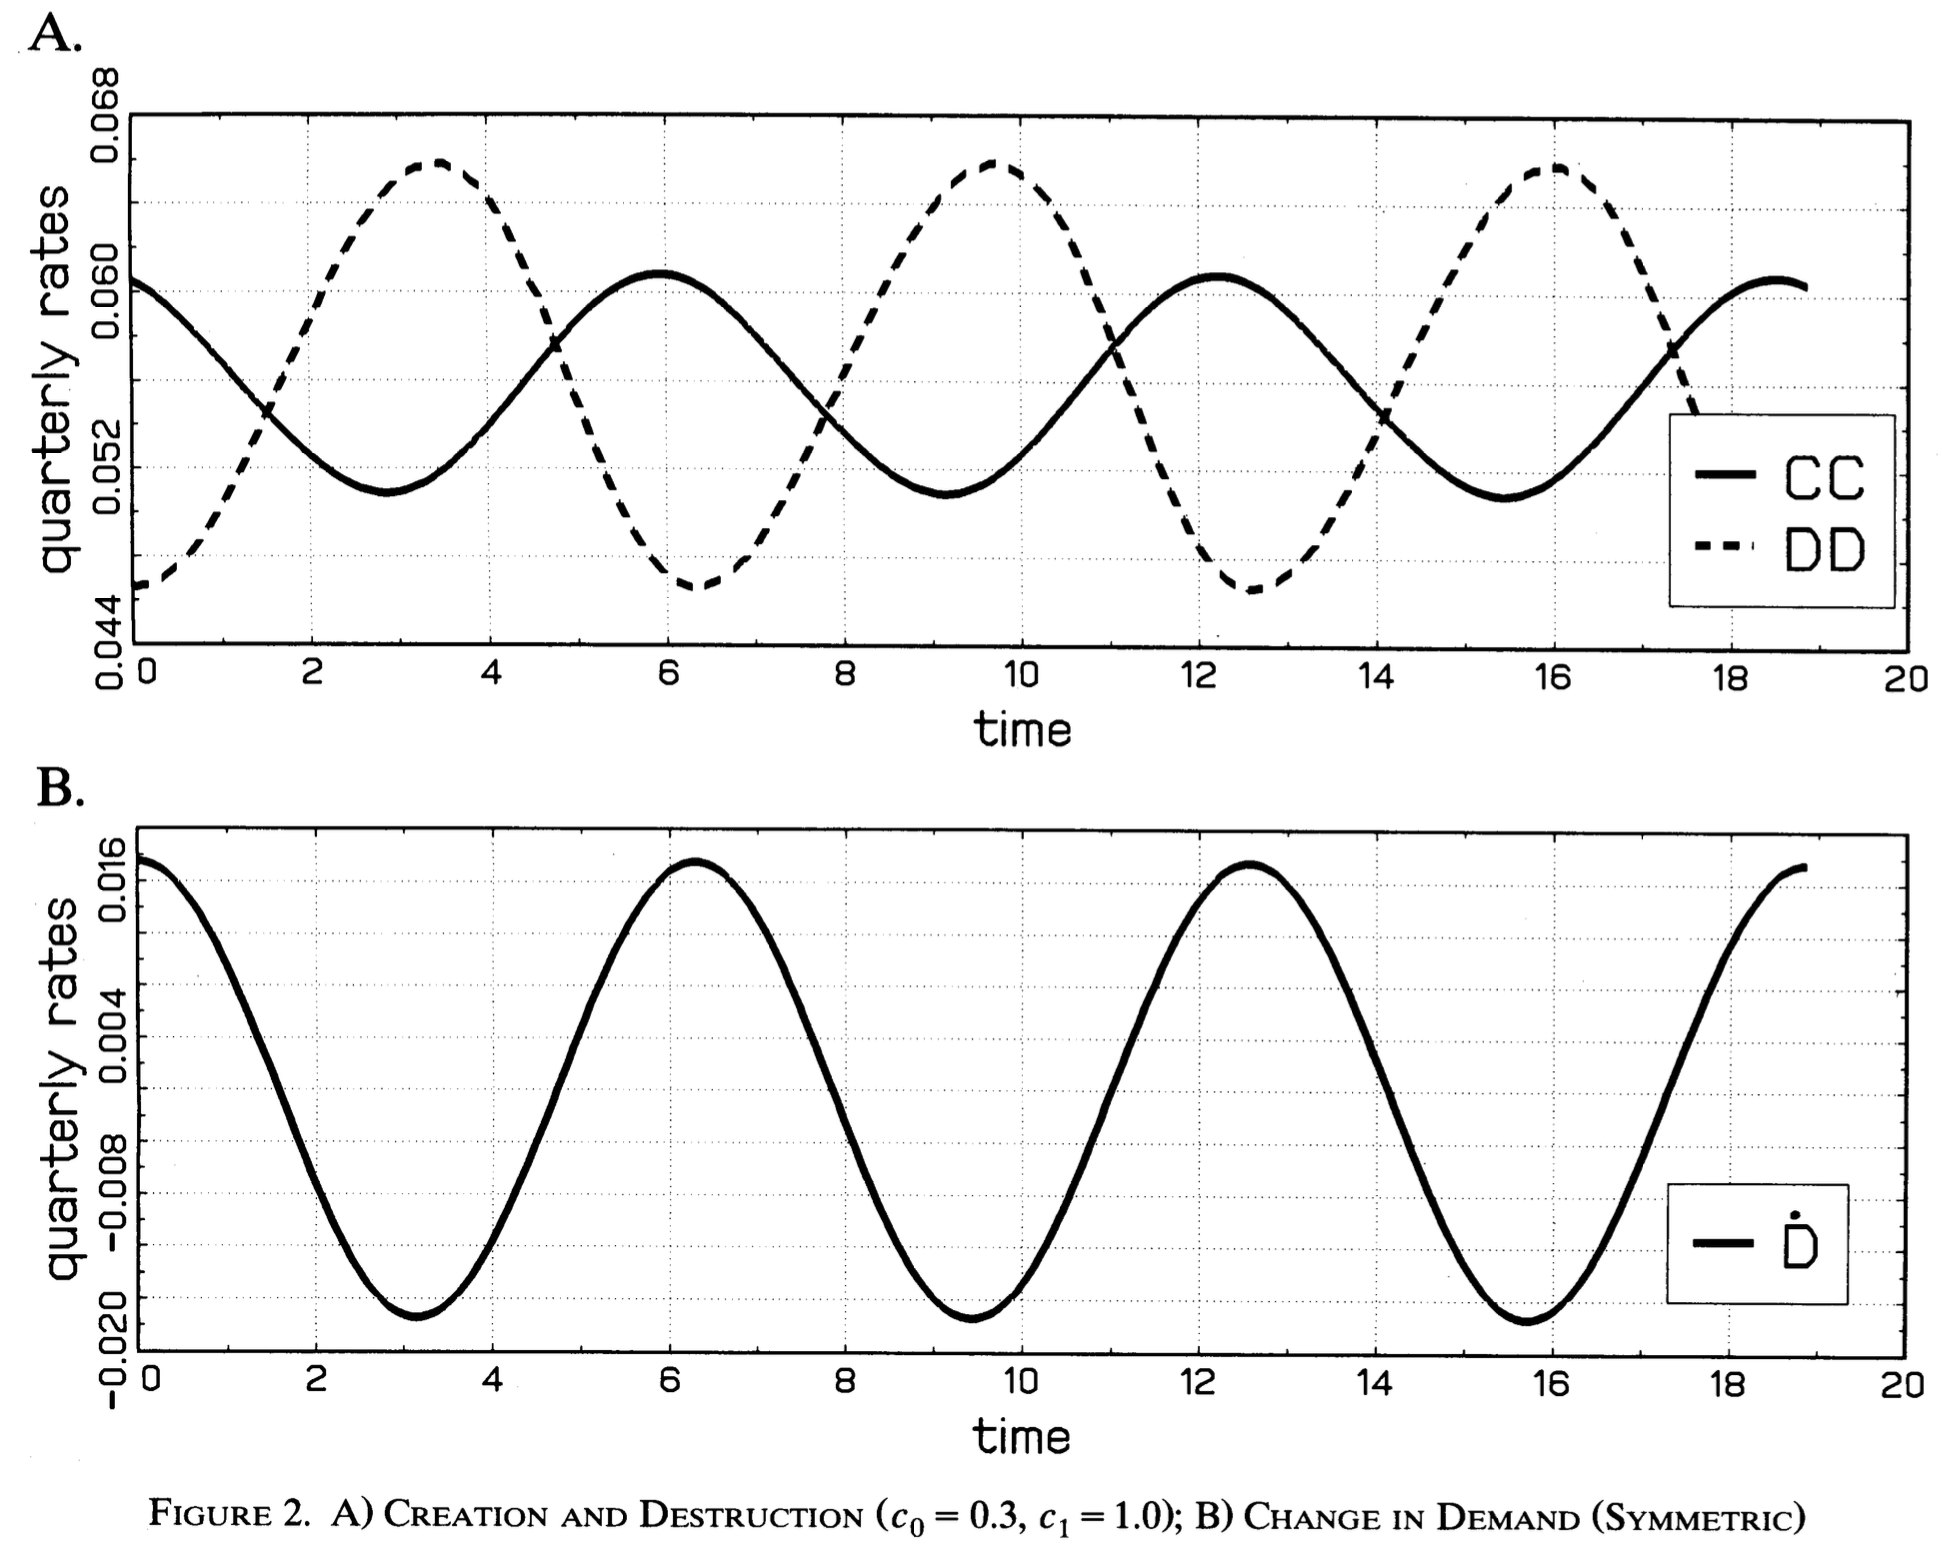
\includegraphics[scale = 0.4]{Plot2.1.png}
    \caption{Figure 1. A Creation and destruction \(c_0=0.3, c_1=1\) B Change in demand (Symmetric)}
    \label{plot:2.1}
\end{figure}

The plot clearly illustrates that the insulation effect is only partial; otherwise, DD would have remained flat, as in
the case with \(c(f(0,t)=c)\). From a mathematical perspective, destruction responds to demand as equations
\ref{eq_2.3}-\ref{eq_2.5} are no longer independent of the path \(f(0,t)\) and demand. From an economic standpoint,
increasing creation costs smoothen the creation process. In scenarios with a nearly flat innovation rate, firms during
crises cannot fully accommodate lower demand, nullifying the adoption of new production units, as the marginal costs
would exceed the reduction in existing production units. \par
In the considered model, production units integrate labor and capital in fixed proportions to generate output. Each unit
can be conceptualized as contributing to job creation within the industry, and job-flow data serves as a metric for
quantifying the flows of production units. 

Datasets that closely align with the theoretical CC and DD series have been compiled by Davis and Haltiwanger
\cite{DAvHalt90,DavHalt92} and Blanchard and Diamond \cite{BlaDia90}, drawing from various sources. The primary focus
lies on the dataset curated by Davis and Haltiwanger, who leverage the Longitudinal Research Database to construct
quarterly series for U.S. manufacturing plants spanning the period 1972:2-1986:4. 

In their empirical approach, Davis and Haltiwanger utilize output to empirically determine demand, employing the growth
rate of the industrial production index as a proxy for output growth. Notably, in the foundational theoretical model,
\(Q(r)\) is smoothed by price movement, with the elasticity of demand determining the extent of smoothing, assumed to be
equal to 1. While the theoretical model maintains a constant consumption-wage, the authors acknowledge that considering
a procyclical consumption-wage, as in the case of general equilibrium with correlated industry shocks, may dampen the
effect of demand shocks. However, they assert that this adjustment would alter only the magnitude, not the direction, of
the analysis. 

The figure below illustrates the data that the model seeks to replicate, showcasing job creation, job destruction, and growth.

\begin{figure}
    \centering
    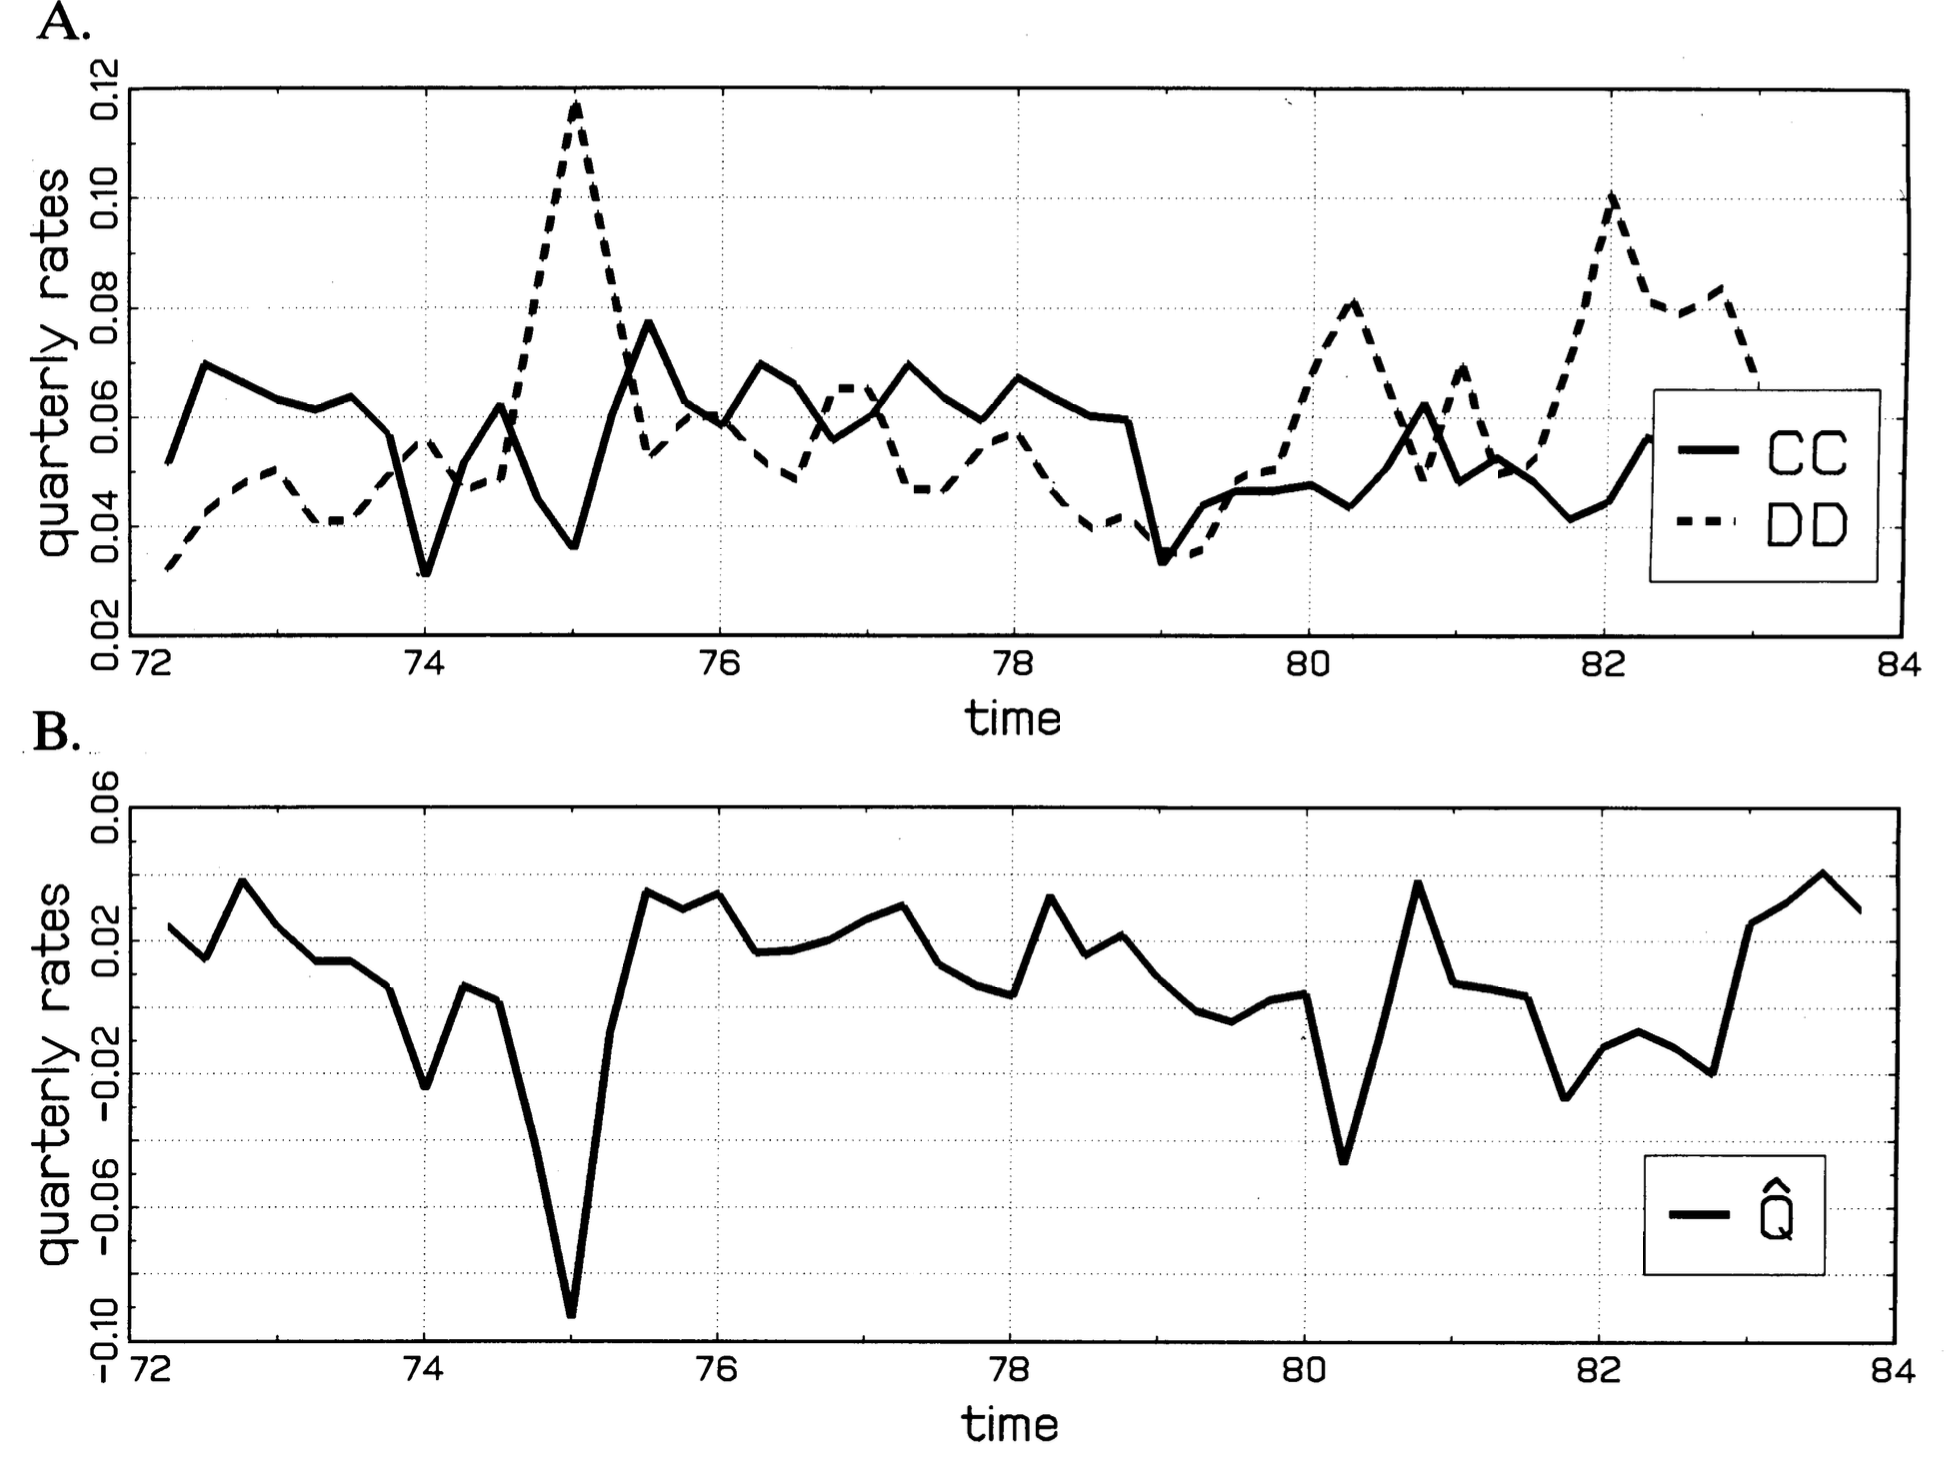
\includegraphics[scale = 0.4]{Plot2.2.png}
    \caption{Figure 1. Job creation and job destruction in U.S. Manufacturing B Index of the industrial production}
    \label{plot:2.2}
\end{figure}

To discern the characteristics of the series, the authors perform regression analysis on sectoral rates of job creation
and job destruction against leads and lags of the corresponding rates of growth. They find that job creation is less
responsive to demand fluctuations, while job destruction exhibits a more countercyclical behavior. 
\begin{figure}
    \centering
    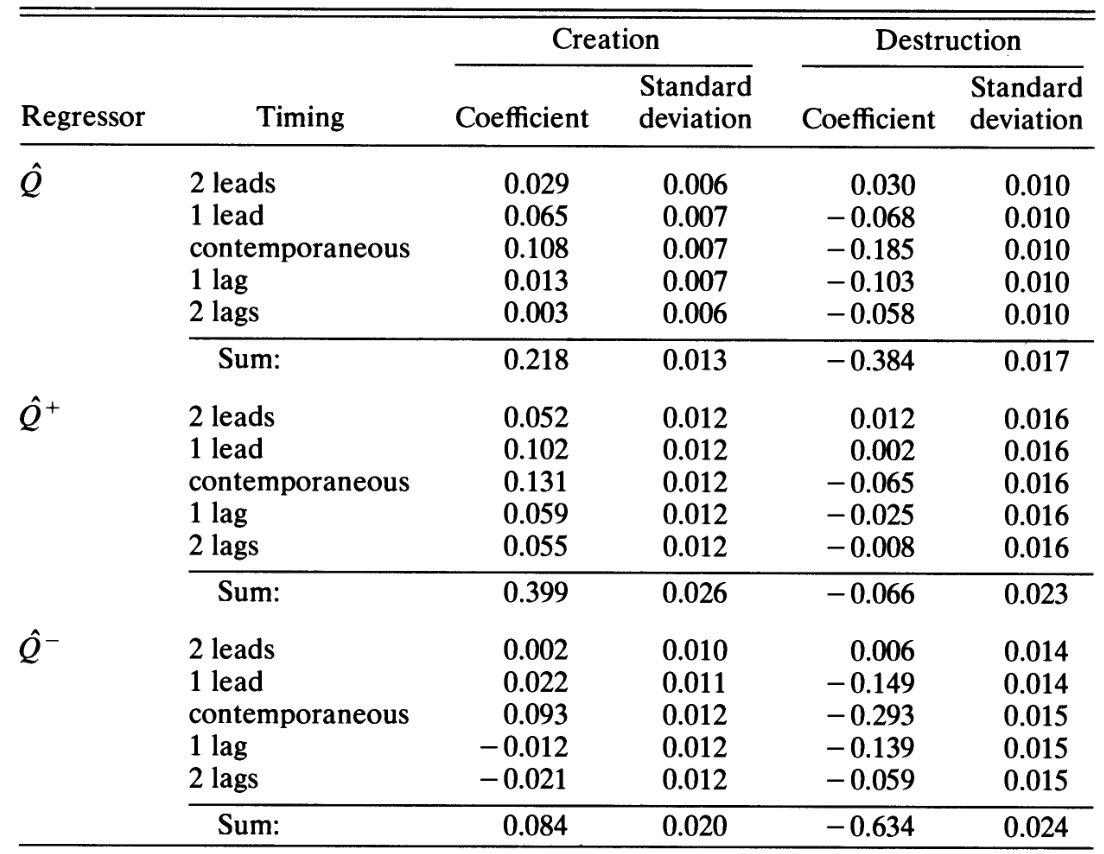
\includegraphics[scale = 0.4]{Plot2.3.png}
    \caption{Table 2.1. Job Creation and Job Destruction in U.S. Manufacturing Response to Output Growth}
    \label{Table 2.1.}
    \footnotesize \textit{Notes}: The table presents the reaction of job creation to the growth rate of the industrial production index. The latter is categorized into values above and below its mean (Q). The table encompasses quarterly observations for the two-digit SIC industries during the period 1972:2-1986:4. The coefficients are uniformly constrained to be equal across all sectors, with the exception of a constant (not shown).
\end{figure}
The initial finding indicates that the rate of job destruction displays greater responsiveness to changes in sectoral
activity compared to the rate of job creation. Specifically, the sums of coefficients are -0.384 for job destruction and
0.218 for job creation showed in the table \ref{Table 2.1.}, the same results as in \cite{DAvHalt90,DavHalt92} and in
\cite{BlaDia90}.
The authors capitalize on a natural experiment rooted in the intrinsic asymmetric characteristics of business cycles.
Recessions, marked by brevity but intense contractions, provide the backdrop for the authors' model. This model
endeavors to emulate the creation rate while concurrently mitigating the impact of asymmetric cyclicality inherent in
business cycles. The empirical evidence supporting this model's behavior is encapsulated in Table \ref{Table 2.1.},
wherein two distinct scenarios are explored: output growth trajectories above \(Q^+\) and below \(Q^-\), relative to
their respective means. The table meticulously delineates how creation and destruction rates respond to these deviations
in output growth. 
\par
The salient observation emerges regarding creation rates, elucidating that they exhibit a more rapid and robust response
in instances of vigorous output growth, as opposed to scenarios where the output growth rate experiences a reduction. On
a contrasting note, the destruction margin, in line with the model's projections, manifests heightened sensitivity to a
decline in output. This responsiveness is particularly pronounced from one quarter before the onset of the shock to one
quarter after. Notably, during expansionary phases, the mean response of the destruction margin is -0.066, a notably
milder reaction compared to the recessionary case where the mean response stands at -0.634. 
\par
These empirical outcomes seamlessly align with the predictions of the model. Specifically, the creation rate exhibits
heightened responsiveness during expansionary phases, given their cyclical and symmetric nature. In contrast, the
asymmetric and non-cyclical nature of recessions triggers a more substantial decline in the production unit rate, in
line with the model's expectations. 
\par 
In oder to better understand the asymmetrical behavior the authors simulate an asymmetrical demand function:
\[\cdot{\overline{D}}(t)=0.05[\cos(t)+\sin(t)] - 0.016 \sin(2t)-0.003\cos(3t)\]
\[\overline{D}(t)=1\quad r = 0.065, \delta =0.15, \gamma=0.028, c_0=0.3, c_1=1.0\] 
The results are depicted in \ref{plot:2.4}
\begin{figure}
    \centering
    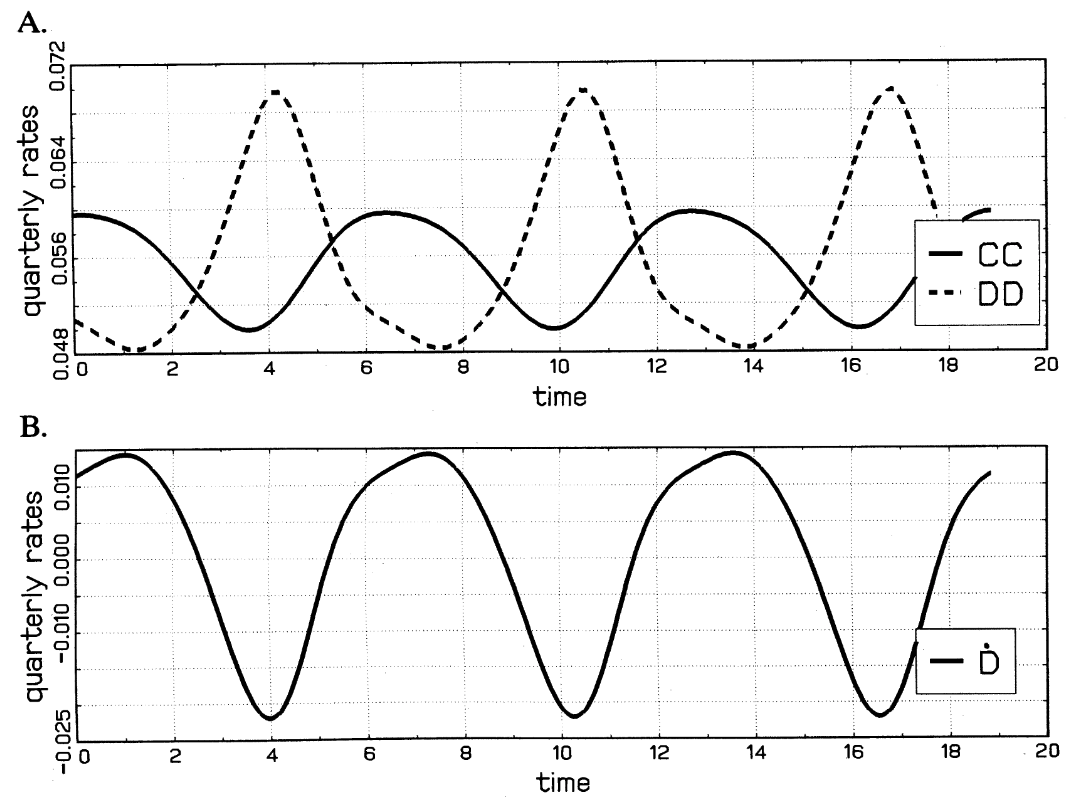
\includegraphics[scale = 0.4]{Plot2.4.png}
    \caption{A.  Creation and  Destruction B. Output Growth}
    \label{plot:2.4}
    \footnotesize \textit{Notes}: The figure depicts a simulation of asymmetrical supply growth.
\end{figure}

From the plot \ref{plot:2.4}, its evident that firms use prediction in demand to smooth job creation in order to avoid
big change, since they are too costly,by avaraging the demand over the lifetime of a production unit ove. On the other
hand, destruction depends only on current conditions, thus responding only to significant deviations from the demand
prediction . It can be better undestand thinking about a case in which creation rates respond only mildy to a sharp
deacrease in demand, the equilibrium price falls leading to additional distruction, since older units' profits go to 0.
Indeed, destruction not only preserves , but amplifies the assymetry of demand.\section{Frictionless economy}
\par
The authors culminate their study with a compelling calibration exercise using manufacturing series to exploit the
model. This entails dissecting the observed net change in employment into destruction and creation rates, as well as
applying the same approach to output production. The model is simulated for the duration of 1972:2-1983:4, with
parameters as follows: 

\begin{equation}
    \begin{aligned}
    &\text { Table 2.1 \label{Tab2.1} - Calibrated Parameters }\\
    &\begin{array}{lcc}
    \hline \hline \text { Variable } & \text { Symbol } & \text { Value } \\
    \hline \text { Interest rate } & r & 0.065 \\
    \text { Depreciation rate } & \delta & 0.150 \\
    \text { Rate of technical progress } & \gamma & 0.028 \\
    \text { Adjustment cost parameters } & c_0 & 0.403 \\
    & c_1 & 0.500 \\
    \hline
    \end{array}
    \end{aligned}
\end{equation}

The technical progress is selected to attribute all the growth in employment and manufacturing to technological
advancements, setting \(\lambda\) as 2.8. The authors employ Equation \ref{eq2.9}, linking the steady state to the
lifetime of jobs and job turnover (\(CC^*\)), determining \(\overline{a}^*+7.42\) years. Utilizing this information,
they ascertain the steady state entry cost to be 0.525, equivalent to half a year's operating costs for production
units. Subsequently, they employ ordinary least squares (OLS) to retrieve the value of \(c_1\), the marginal cost of
creating a new unit, which is found to be 0.5. This aligns with a small elasticity for the creation cost function,
signifying the vulnerability of the insulation mechanism to breakdown. 
\begin{figure}
    \centering
    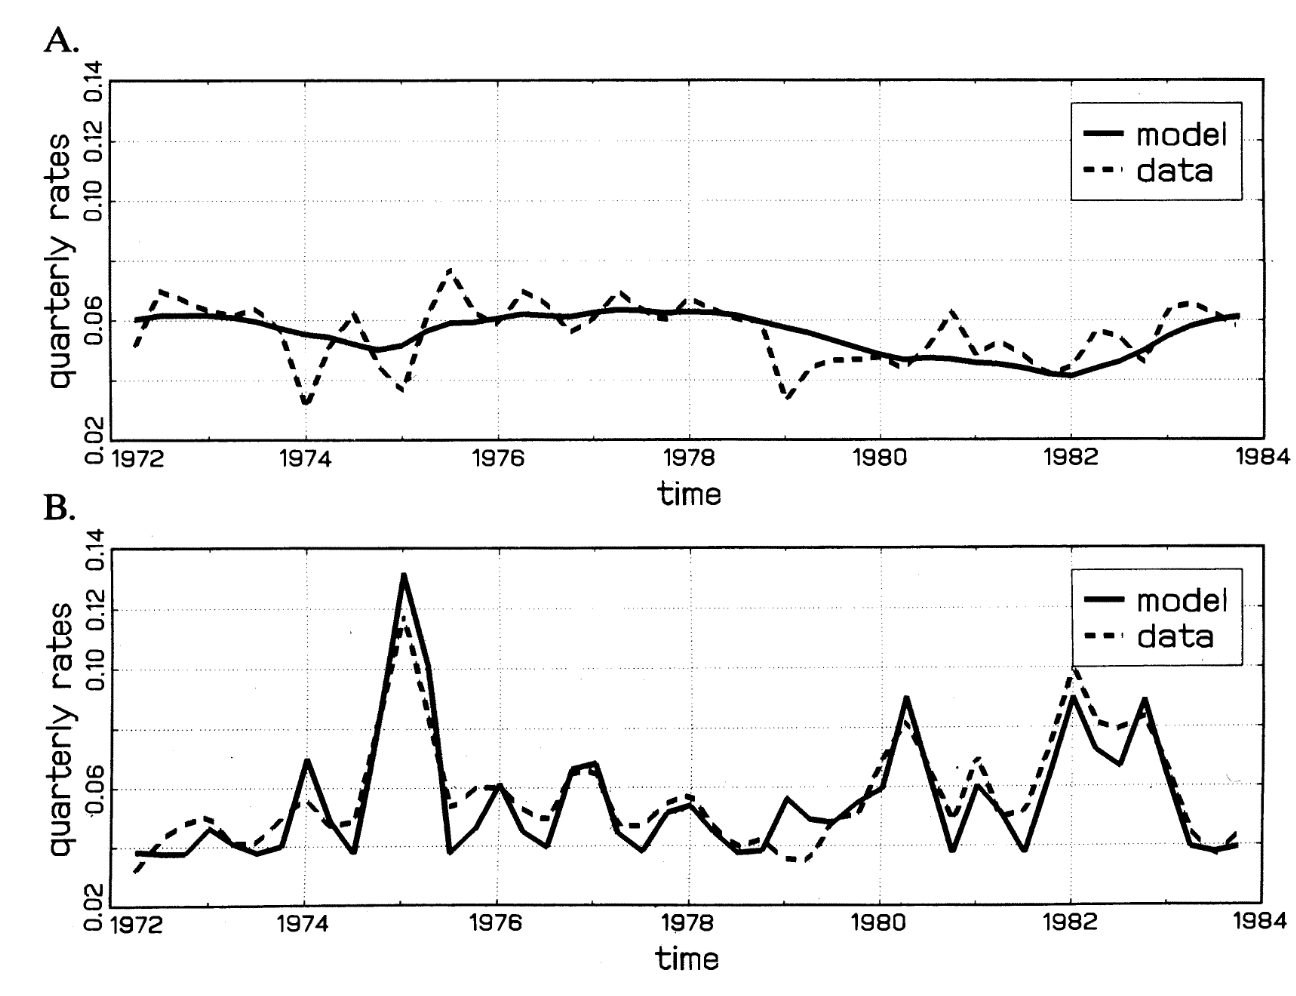
\includegraphics[scale = 0.4]{Plot2.5.png}
    \caption{Figure 1. A employment driven job creation \(c_0=0.403, c_1=0.5\) B Employment job destruction \(c_0=0.403, c_1=0.5\)} 
    \label{plot:2.5}
\end{figure}
The outcomes stemming from the simulations driven by employment and output are disclosed and contrasted with the data in
Figure \ref{plot:2.5}. Notably, the simulation of job creation displays a level of smoothness that diverges from the
observed 
data, with this discrepancy being attributed, in part, to the inherent absence of uncertainty in our model. Despite
this, the model effectively elucidates the relative volatility discernible in the patterns of job creation and
destruction. Moreover, it successfully captures the greater symmetry observed in the former, offering insights into the
nuanced dynamics at play in employment and output fluctuations. 

\section{Solving}

Given that the evolution of the net worth is the following:
\[e_{t+1} = Z(\theta +\epsilon)k_t^\alpha + (1-\delta )k_t - (1+r)(c+k_t-e_t)\]
The value of the firm at time t is given by:
\[V_t(e_t) =\max_{k_t}  e_t + \beta V_{t+1}(e_{t+1})\]

Solving the Belman equation, the FOC are given by:
\[\frac{\vartheta V_t(e_t)}{\vartheta k_t } =\frac{\vartheta e_t}{\vartheta k_t } +
 \beta \frac{\vartheta V_{t+1}(e_{t+1})}{\vartheta k_t } \]
Strong assumption a change in \(k_t\) does not have an impact on \(e_t\) only on \(e_{t+1}\):
\[\frac{\vartheta e_t}{\vartheta k_t} = 0\]
Using the envelope theorem:
\[\frac{\vartheta
V_{t+1}(e_{t+1})}{\vartheta k_t } = \frac{\vartheta
V_{t+1}(e_{t+1})}{\vartheta e_{t+1} }\frac{\vartheta e_{t+1}}{\vartheta k_t}\]
\[\frac{\vartheta V_{t+1}(e_{t+1})}{\vartheta e_{t+1} } =1 + \beta(1+r)\]
\[\frac{\vartheta e_{t+1}}{\vartheta k_t} = Z(\theta +\epsilon)\alpha k_t^{\alpha-1}
-(\delta + r)\]
Thus:
\[\frac{\vartheta V_{t+1}(e_{t+1})}{\vartheta k_t } = 
[1+\beta(1+r)] [Z(\theta + \epsilon)\alpha k_t^{\alpha-1}-(\delta + r)] \]
So the FOC became:
\[\frac{\vartheta V_t(e_t)}{\vartheta k_t } = 0 + \beta [1+\beta(1+r)] [Z(\theta + \epsilon)\alpha
k_t^{\alpha-1}-(\delta + r)]  = 0 \]
The optimal level of capital at time t is:
\[\widehat{k} _t= {\frac{\beta(1+r) Z(\theta +\epsilon)\alpha}{\delta + r}}^{\frac{1}{1-\alpha}} \]
Plotting the graph in (assuming \(X=Z(\theta +\epsilon)\)) and \(y=\widehat{k} _t\)
\[ y={\frac{0.8 x}{0.03+0.1}}^{\frac{1}{1-0.8}}\]

\begin{figure}
    \centering
    \includegraphics[scale = 0.8]{K.png}
    \caption{\(X=Z(\theta +\epsilon)\) and \(y=\widehat{k} _t\) }
    \label{plot:k_static}
\end{figure}
Its interesting to see that if there is an increase in productivity the firm need more optimal capital K, while the most
low productivity firms need less capital to operate 


\subsection{Frictions}
Now I consider the participation constraint of the borrower given that she could observe \(\epsilon\) only paying \(\mu
k^\alpha\) so:
\[
 (1+r )(k+c+e)(1-\Phi(\overline{\epsilon}))+\int_{-\infty}^{\overline{\epsilon}}[Z(\theta+\overline{\epsilon})
k^\alpha+(1-\delta)k-\mu k^\alpha] \,d\Phi(\epsilon) \geq (1+r)(c+k+e)
 \]
\(r\) is the rate of interest that makes equal the expected value of borrowing to the opportunity cost of capital.
rewriting became 
\[
Z[\theta+G(\overline{\epsilon} )]k_t^\alpha+(1-\delta)k_t-uk_t^\alpha\Phi (\overline{\epsilon})=(1+r)(k_t+c-e_t)
\]
where
\[G(\overline{\epsilon} )= (1-\Phi(\varepsilon )\overline{\varepsilon }
+\int_{-\infty}^{\overline{\varepsilon}}\epsilon\,d \Phi(\epsilon) )\]
While the firm participation constraint is \(q_t \geq 0 \) so the end-of-period net worth must be greater than 0, thus
the problem of the firm becomes:
The value of the firm at time t is given by:
\[V_t(e_t) =\max_{k_t}  q_t - e_{t+1} + \beta V_{t+1}(e_{t+1})\]
\[s.t.\]
\[q_{t} = Z(\theta +\epsilon)k_t^\alpha + (1-\delta )k_t - (1+r)(c+k_t-e_t)\]
\[
Z[\theta+G(\overline{\epsilon} )]k_t^\alpha+(1-\delta)k_t-uk_t^\alpha\Phi (\overline{\epsilon})=(1+r)(k_t+c-e_t)
\]
so we can rewrite the second constraint in order to get \(r\):
\[r = \frac{Z[\theta+G(\overline{\epsilon} )]k_t^\alpha+(1-\delta)k_t-uk_t^\alpha\Phi (\overline{\epsilon})}{k_t+c-e_t}-1\]
FOC:
\[\frac{\vartheta
V_{t}(e_{t})}{\vartheta k_t } = \frac{\vartheta
q_{t}}{\vartheta k_t } - \frac{\vartheta
e_{t}}{\vartheta k_t } + \beta \frac{\vartheta
V_{t+1}(e_{t+1})}{\vartheta k_{t} } = 0\]
by envelope theorem:
\[\frac{\vartheta
V_{t+1}(e_{t+1})}{\vartheta k_{t} } = \frac{\vartheta
V_{t+1}(e_{t+1})}{\vartheta e_{t+1} }\frac{\vartheta e_{t+1}}{\vartheta k_t}\]
Strong HP: \[\frac{\vartheta e_{t+1}}{\vartheta k_t} = 0\]
Qui non so se ha senso continuare perchè non ho nessun meccanismo che mi trasformi il net worth al tempo t in net worth
al periodo t+1, almeno che non includa la definzione di dividendo come \(d_t= q_t-e_{t+1}\), allora in questo caso
dovrei risolvere il problema con un langrangiana dato che la firm dovrebbe scegliere sia \(k\) che \(e\) net worth.
\section{Redefining the problem}
\[V(k_{t}) = \max_{k_{t+1}, e_{t+1}} d_t + \beta V(k_{t+1})\]
\[s.t.\]
\[f(k_t) = Z k_t^\alpha\]
\[f(k_t) = d_t + (c+k_{t-1}-e_{t-1})(1+r) + k_{t} - (c + k_{t}- e_{t}) - k_{-1}(1-\delta)\]
\[(1+r)(c+k_t -e_t)p + (1-p)f(k_t) = (1+r_f)(c+k_t -e_t) \]
\[B_t = c+k_t-e_t; R= 1+r; R_f= 1 + r_f;  \]
\[R=\frac{R_f}{p}  -\frac{ 1-p }{ p }\frac{f(k_t)}{D_t}\]
In order to understand the mechanism behind this optimization problem, I firstly solve the three times problem working
backward.
The value function in \(t=2\) is 
\[ V_{t+2} =  \max d_{t+2}\]
Since there firm will not exists in t+2, there are no investiment \(B_{t+2}=0\), thus \(0=k_{t+2}+c-e_{t+2}\) as
consequence \(k_{t+2} = e_{t+2} - c\). Then we can rewrite the value function:
\[ V_{t+2} = \max Z(e_{t+2} - c)^\alpha - (c+k_{t+1}-e_{t+1})(1+r_{t+1}) - e_{t+2} + c + (c + e_{t+2} - c - e_{t+2}) +
k_{t+1}(1-\delta) \]
\[V_{t+2} = \max_{e_{t+2}} Z(e_{t+2} - c)^\alpha - B_{t+1}R_{l,t+1} - e_{t+2} + c + k_{t+1}(1-\delta) \]
FOC:
\[\frac{\partial V_{t+2}}{\partial e_{t+2}} = Z \alpha (e_{t+2} - c)^{\alpha-1} - 1 = 0\]
\[ (e_{t+2} - c)^{\alpha-1}= (Z \alpha)^{-1}\]
\[ e_{t+2} = (Z \alpha)^{\frac{1}{1-\alpha}}+c\]
Thus:
\[d_{t+2} = Z\left[(Z \alpha)^{\frac{\alpha}{1-\alpha}}\right]  - B_{t+1}R_{t+1} -  \left[(Z
\alpha)^{\frac{1}{1-\alpha}}\right] + k_{t+1}(1-\delta) \]
\[V_{t+2} = Z\left[(Z \alpha)^{\frac{\alpha}{1-\alpha}}\right]  - B_{t+1}R_{t+1} -  \left[(Z
\alpha)^{\frac{1}{1-\alpha}}\right] + k_{t+1}(1-\delta) \]
Writing the problem in t+1:
\[V_{t+1} = \max_{e_{t+1},k_{t+1}} d_{t+1} + \beta V_{t+2}\]
\[d_{t+1} = Zk^\alpha_{t+1} - B_t R_L - k_{t+1} + B_{t+1} + k_t(1-\delta)\]
FOCs:
\begin{equation}
    \left\{\begin{array}{@{}l@{}}
        \frac{\partial V_{t+1}}{\partial e_{t+1}} = \frac{\partial d_{t+1}}{\partial e_{t+1}} + \beta \frac{\partial
            V_{t+2}}{\partial e_{t+1}} = 0  \\
        \frac{\partial V_{t+1}}{\partial k_{t+1}} = \frac{\partial d_{t+1}}{\partial k_{t+1}} + \beta \frac{\partial
            V_{t+2}}{\partial K_{t+1}} = 0 \\
    \end{array} \right .\,
\end{equation}
solving \(\frac{\partial d_{t+1}}{\partial e_{t+1}}\):
\[\frac{\partial d_{t+1}}{\partial e_{t+1}} = Z \alpha k_{t+1} ^{\alpha-1}\frac{\partial k_{t+1}}{\partial e_{t+1}}
 - \frac{\partial k_{t+1}}{\partial e_{t+1}} + \frac{\partial B_{t+1}}{\partial e_{t+1}}\]
\[\frac{\partial B_{t+1}}{\partial e_{t+1}} = \frac{\partial k_{t+1}}{\partial e_{t+1}} - 1\]
\[\frac{\partial d_{t+1}}{\partial e_{t+1}} = Z \alpha k_{t+1} ^{\alpha-1}\frac{\partial k_{t+1}}{\partial e_{t+1}} -
\frac{\partial k_{t+1}}{\partial e_{t+1}} + \frac{\partial k_{t+1}}{\partial e_{t+1}} - 1\]

solving \(\frac{\partial V_{t+2}}{\partial e_{t+1}}\):
\[\frac{\partial V_{t+2}}{\partial e_{t+1}} = - \left[\frac{\partial B_{t+1}R_{t+1}}{\partial e_{t+1}} - \frac{\partial
k_{t+1}}{\partial e_{t+1}} \left( 1-\delta \right) \right]\] 
\[\frac{\partial B_{t+1}R_{t+1}}{\partial e_{t+1}} = \frac{\partial B_{t+1}}{\partial e_{t+1}}R_{t+1} +
B_{t+1}\frac{\partial R_{t+1}}{\partial e_{t+1}} \]
\[\frac{\partial B_{t+1}}{\partial e_{t+1}} = \frac{\partial k_{t+1}}{\partial e_{t+1}}-1\]
\[\frac{\partial R_{t+1}}{\partial e_{t+1}} = - \frac{1-p}{p}\left\{\left[Z\alpha k^{\alpha-1}_{t+1}\frac{\partial
k_{t+1}}{\partial e_{t+1}} -\delta \frac{\partial k_{t+1}}{\partial e_{t+1}}\right] B_{t+1} - \left(\frac{\partial
k_{t+1}}{\partial e_{t+1}} - 1\right) \left[Zk_{t+1}^{\alpha} - \delta k_{t+1}\right]\right\}B_{t+1}^{-2}\]
\[\frac{\partial B_{t+1}R_{t+1}}{\partial e_{t+1}} = \left[\frac{\partial k_{t+1}}{\partial e_{t+1}}-1 \right] R_{t+1}
- \frac{1-p}{p}\left\{\left[Z\alpha k^{\alpha-1}_{t+1}\frac{\partial
k_{t+1}}{\partial e_{t+1}} -\delta \frac{\partial k_{t+1}}{\partial e_{t+1}}\right] B_{t+1} - \left(\frac{\partial
k_{t+1}}{\partial e_{t+1}} - 1\right) \left[Zk_{t+1}^{\alpha} - \delta k_{t+1}\right]\right\}B_{t+1}^{-1}\]
\[\frac{\partial B_{t+1}R_{t+1}}{\partial e_{t+1}} = \left(\frac{\partial k_{t+1}}{\partial e_{t+1}} -1
\right)\left[\left(zk^\alpha_{t+1} -\delta k_{t+1}\right)\frac{1-p}{p}B_{t+1}^{-1}+R_{t+1}\right] -
\frac{1-p}{p}\frac{\partial k_{t+1}}{\partial e_{t+1}} \left(Z\alpha k^{\alpha-1}_{t+1} - \delta\right)\]
\[\frac{\partial B_{t+1}R_{t+1}}{\partial e_{t+1}} = \left(\frac{\partial k_{t+1}}{\partial e_{t+1}} -1
\right)R_f-
\frac{1-p}{p}\frac{\partial k_{t+1}}{\partial e_{t+1}} \left(Z\alpha k^{\alpha-1}_{t+1} - \delta\right)\]
\[\frac{\partial V_{t+2}}{\partial e_{t+1}} = - \left[\left(\frac{\partial k_{t+1}}{\partial e_{t+1}} -1
\right)R_f-
\frac{1-p}{p}\frac{\partial k_{t+1}}{\partial e_{t+1}} \left(Z\alpha k^{\alpha-1}_{t+1} - \delta\right) - \frac{\partial
k_{t+1}}{\partial e_{t+1}} \left( 1-\delta \right)\right]\]
Substituting into the first FOC, we get:
\[\frac{\partial V_{t+1}}{\partial e_{t+1}} = Z \alpha k_{t+1} ^{\alpha-1}\frac{\partial k_{t+1}}{\partial e_{t+1}} -
\frac{\partial k_{t+1}}{\partial e_{t+1}} + \frac{\partial k_{t+1}}{\partial e_{t+1}} - 1 - \beta 
\left[\left(\frac{\partial k_{t+1}}{\partial e_{t+1}} -1 
\right)R_f-
\frac{1-p}{p}\frac{\partial k_{t+1}}{\partial e_{t+1}} \left(Z\alpha k^{\alpha-1}_{t+1} - \delta\right) - \frac{\partial
k_{t+1}}{\partial e_{t+1}} \left( 1-\delta \right)\right] = 0\]
second FOC: \\
solving \(\frac{\partial d_{t+1}}{\partial k_{t+1}}\):
\[\frac{\partial d_{t+1}}{\partial k_{t+1}} = Z \alpha k_{t+1} ^{\alpha-1} - 1 + \frac{\partial B_{t+1}}{\partial
k_{t+1}} \]
\[\frac{\partial B_{t+1}}{\partial
k_{t+1}} = 1 - \frac{\partial e_{t+1}}{\partial k_{t+1}} \]
\[\frac{\partial d_{t+1}}{\partial k_{t+1}} = Z \alpha k_{t+1} ^{\alpha-1} - \frac{\partial e_{t+1}}{\partial
k_{t+1}}\]
solving \(\frac{\partial V_{t+2}}{\partial k_{t+1}}\):
\[\frac{\partial V_{t+2}}{\partial k_{t+1}} = -\left[\frac{\partial B_{t+1}R_{t+1}}{\partial k_{t+1}} -(1-\delta)\right] \]
\[\frac{\partial B_{t+1}R_{t+1}}{\partial k_{t+1}} = \frac{\partial B_{t+1}}{\partial k_{t+1}}R_{t+1} +
B_{t+1}\frac{\partial R_{t+1}}{\partial k_{t+1}}\]
\[\frac{\partial B_{t+1}}{\partial k_{t+1}} = 1-\frac{\partial e_{t+1}}{\partial k_{t+1}} \]
\[\frac{\partial R_{t+1}}{\partial k_{t+1}} =  - \frac{1-p}{p}\left[\left(Z\alpha k^{\alpha-1}_{t+1}-\delta\right)B_{t+1} -
\left(1-\frac{\partial e_{t+1}}{\partial k_{t+1}}\right)\left(Zk_{t+1}^{\alpha} - \delta k_{t+1}
\right)\right]B_{t+1}^{-2} 
\]
\[\frac{\partial B_{t+1}R_{t+1}}{\partial k_{t+1}} = \left(1-\frac{\partial e_{t+1}}{\partial k_{t+1}}\right) R_{t+1} +
\left\{\frac{1-p}{p}\left[(Z \alpha k^{\alpha-1}_{t+1}-\delta)B_{t+1} -
\left(1-\frac{\partial e_{t+1}}{\partial k_{t+1}}\right)\left(Zk_{t+1}^{\alpha} - \delta k_{t+1}
\right)\right]B_{t+1}^{-1} \right\}\]
\[\frac{\partial B_{t+1}R_{t+1}}{\partial k_{t+1}} =\left(1-\frac{\partial e_{t+1}}{\partial k_{t+1}}\right)
\left[R_{t+1} + \frac{1-p}{p}\left(Z k_{t+1}^{\alpha} - \delta k_{t+1}\right)B_{t+1}^{-1}\right]-
\frac{1-p}{p}\left(Z\alpha k^{\alpha-1}_{t+1}-\delta\right) \]
\[\frac{\partial B_{t+1}R_{t+1}}{\partial k_{t+1}} =\left(1-\frac{\partial e_{t+1}}{\partial k_{t+1}}\right)
R_f - \frac{1-p}{p}\left(Z\alpha k^{\alpha-1}_{t+1}-\delta\right) \]
\[\frac{\partial V_{t+2}}{\partial k_{t+1}} = -\left[\left(1-\frac{\partial e_{t+1}}{\partial k_{t+1}}\right)
R_f - \frac{1-p}{p}\left(Z\alpha k^{\alpha-1}_{t+1}-\delta\right)- \left(1-\delta\right)\right] \]
Substituting into the FOC:
\[\frac{\partial V_{t+1}}{\partial k_{t+1}} =Z \alpha k_{t+1} ^{\alpha-1} - \frac{\partial e_{t+1}}{\partial
k_{t+1}} - \beta \left[\left(1-\frac{\partial e_{t+1}}{\partial k_{t+1}}\right)
R_f - \frac{1-p}{p}\left(Z\alpha k^{\alpha-1}_{t+1}-\delta\right)- \left(1-\delta\right)\right]=0\]
thus the FOCs are:
\[\frac{\partial V_{t+1}}{\partial e_{t+1}} = Z \alpha k_{t+1} ^{\alpha-1}\frac{\partial k_{t+1}}{\partial e_{t+1}}  - 1 - \beta 
\left[\left(\frac{\partial k_{t+1}}{\partial e_{t+1}} -1 
\right)R_f-
\frac{1-p}{p}\frac{\partial k_{t+1}}{\partial e_{t+1}} \left(Z\alpha k^{\alpha-1}_{t+1} - \delta\right) - \frac{\partial
k_{t+1}}{\partial e_{t+1}} \left( 1-\delta \right)\right] = 0\]
\[\frac{\partial V_{t+1}}{\partial k_{t+1}} =Z \alpha k_{t+1} ^{\alpha-1} - \frac{\partial e_{t+1}}{\partial
k_{t+1}} - \beta \left[\left(1-\frac{\partial e_{t+1}}{\partial k_{t+1}}\right)
R_f - \frac{1-p}{p}\left(Z\alpha k^{\alpha-1}_{t+1}-\delta\right)- \left(1-\delta\right)\right]=0\]
rearranging \(\frac{\partial V_{t+1}}{\partial k_{t+1}} \) to isolate \(k_{t+1}\):
\[k^{\alpha-1}_{t+1}=\left[\frac{\partial e_{t+1}}{\partial k_{t+1}}\left(1-\beta R_f\right) + \beta
\left(r_f+\frac{\delta}{p}\right)\right]\left\{Z\alpha\left[\left(1-\beta\right)-\frac{\beta}{p}\right]\right\}^{-1}\] 
rearranging \(\frac{\partial V_{t+1}}{\partial e_{t+1}} \) to isolate \(k_{t+1}\):
\[k^{\alpha-1}_{t+1}=\left[\frac{\partial k_{t+1}}{\partial e_{t+1}}\left(1-\beta R_f\right) + \beta
\left(r_f+\delta\right) + \delta \frac{1-p}{p}\right]\frac{p}{Z\alpha}\]
Equating the two equations:
\[\left[\frac{\partial e_{t+1}}{\partial k_{t+1}}\left(1-\beta R_f\right) + \beta
\left(r_f+\frac{\delta}{p}\right)\right]\left\{Z\alpha\left[\left(1-\beta\right)-\frac{\beta}{p}\right]\right\}^{-1} =
\left[\frac{\partial k_{t+1}}{\partial e_{t+1}}\left(1-\beta R_f\right) + \beta 
\left(r_f+\delta\right) + \delta \frac{1-p}{p}\right]\frac{p}{Z\alpha}\]
From this equation, you can isolate \(\frac{\partial e_{t+1}}{\partial k_{t+1}}\) to solve for it explicitly.
\[\frac{\partial e_{t+1}}{\partial k_{t+1}} = -\left[\frac{\partial k_{t+1}}{\partial e_{t+1}}\left(1-\beta R_f\right) + \beta
\left(r_f+\delta\right) + \delta
\frac{1-p}{p}\right]\frac{p}{Z\alpha}\left\{Z\alpha\left[\left(1-\beta\right)-\frac{\beta}{p}\right]\right\}\left(1-\beta
R_f\right)^{-1} - \beta \left(r_f+\frac{\delta}{p}\right)\left(1-\beta R_f\right)^{-1}\] 
\[\frac{\partial e_{t+1}}{\partial k_{t+1}} =- \left[\frac{\partial k_{t+1}}{\partial e_{t+1}}\left(1-\beta R_f\right)
+\delta\frac{1-p}{p}\right]\frac{\beta p +\beta -p}{1-\beta R_f} - \beta \left(r_f+\frac{\delta}{p}\right)\left(1-\beta
R_f\right)^{-1} \]
Fino a qui non ho molti dubbi, mentre il seguente passaggio presenta molti dubbi e secondo me è responsabile del segno
negativo del capitale. Tuttavia non mi è venuto in mente altro modo per procedere.
Knowing that \(B = k + c - e \rightarrow e= B -k -c\) thus \(\frac{\partial e_{t+1}}{\partial k_{t+1}} = -1\):
\[  -\beta \left(r_f+\frac{\delta}{p}\right)\left(1-\beta R_f\right)^{-1}\frac{1-\beta R_f}{\beta p +\beta -p}= \left[\frac{\partial k_{t+1}}{\partial e_{t+1}}\left(1-\beta R_f\right)
+\delta\frac{1-p}{p}\right]\]


We can rearrange it to isolate \(\frac{\partial k_{t+1}}{\partial e_{t+1}}\):

\[ -\beta \left(r_f+\frac{\delta}{p}\right)\left(\beta p +\beta -p\right) - \delta\frac{1-p}{p} = \frac{\partial k_{t+1}}{\partial e_{t+1}}\left(1-\beta
R_f\right)\] 

Now, solve for \(\frac{\partial k_{t+1}}{\partial e_{t+1}}\) by dividing both sides by \((1-\beta R_f)\):

\[\frac{\partial k_{t+1}}{\partial e_{t+1}} = \left\{-\beta \left(r_f+\frac{\delta}{p}\right)\left(\beta p +\beta
-p\right) - \delta\frac{1-p}{p} 
\right \} \left(1-\beta R_f\right)^{-1}\]

This equation provides the value of \(\frac{\partial k_{t+1}}{\partial e_{t+1}}\) in terms of the given constants
(\(\beta, R_f, p, \delta\)) and the relationship between \(e_{t+1}\) and \(k_{t+1}\). 
\[k^{\alpha-1}_{t+1}=\left[\left\{-\beta \left(r_f+\frac{\delta}{p}\right)\left(\beta p +\beta
-p\right) - \delta\frac{1-p}{p} 
\right \} + \beta
\left(r_f+\delta\right) + \delta \frac{1-p}{p}\right]\frac{p}{Z\alpha}\]
\[k^{\alpha-1}_{t+1}= \left[\left\{-\beta \left(r_f+\frac{\delta}{p}\right)\left(\beta p +\beta
-p\right) 
\right \} + \beta
\left(r_f+\delta\right) \right]\frac{p}{Z\alpha}\]
\medskip

\bibliography{reference}


\end{document}